\section{Models}

\subsection{AlexNet}
\citeauthor{Krizhevsky2012} have presented their influential \emph{AlexNet} in \citeyear{Krizhevsky2012}. It consists of only five convolutional layers, some additional max-pooling layers and three fully connected layers at the end, so its structure is rather simple. Nonetheless, it is packed with more than 40.000.000 trainable parameters (the fully connected layers at the end are very large), making it not exactly computationally cheap to train. An AlexNet was supposed to serve as our baseline model from which we wanted to build things up.

\subsection{EfficientNet}
We then implemented a pre-trained EfficientNet with custom top layer. The EfficientNet model family was first introduced in 2019 (\citeauthor{Tan2019}) with the idea of providing scalable CNN architectures. Multiple networks of different size for image classification purposes were introduced, many achieving better results than state-of-the-art models like MobileNet and ResNet while being significantly smaller in terms of depth, width, and image resolution \citep{Tan2019}. Two years later, a second, even more powerful and efficient generation was introduced: EfficientNetV2 \citep{Tan2021}. For our purposes, given the low input resolution of $224\times224$, the model of choice is the EfficientNetV2-B0 -- the smallest model of the ensemble. The model is pre-trained on ImageNet21k and we implemented a custom fully-connected layer at the end to match our classification task.

\subsection{InceptionNet}
For an additional comparison, we implemented yet another supposedly very efficiently designed CNN, the InceptionV3 as introduced by \citeauthor{Szegedy2015} in \citeyear{Szegedy2015}. Its computational low cost makes the Inception architecture an attractive choice when resources are limited, e.g. in mobile scenarios. The inception network was a milestone in the development of CNN classifiers. It achieved extremely high accuracies on the ImageNet dataset for example the inception v3 network achieved an accuracy of 78,1 percent. 
The fundamental idea behind the inception network is the inception block. In a traditional convolutional neural network layer, the previous layer's output is the input of the next layer until the state of prediction is accomplished. The inception block takes apart the individual layers. The previous layer's output is passed to four different operations in parallel and concatenates the outputs from all these different layers. So instead of constructing a deeper network, a “ wider network” is provided. The naive approach consists of a 1x1 convolution layer, a 3x3 convolution layer and a 5x5 convolutions layer followed by a max-pooling layer and a concatenation layer. Due to the high computational cost especially with the 5x5 filter, the 1x1 is first added to the naive inception module. This leads to a computational reduction of 90 percent.
Additionally, the 1x1 convolutional filters allow learning cross channel patterns across the depth of the input data. 


%picture of Convolution 
\begin{figure}[htb]
    \centering
    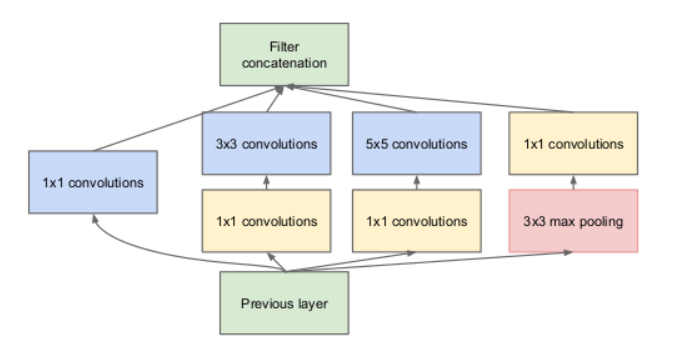
\includegraphics[width=7cm]{images/InceptionNet.jpg}
    \caption{Inception Block}
    \label{fig:incepblock}
\end{figure}


- balance of depth and width within network
- aggressive regularisation
- inception architecture already introduced by GoogLeNet (2014)


\subsection{Hyperparameters}
For simplicity, we use more or less the same hyperparameters for all networks.

Categorical cross-entropy: Cross-entropy loss is differentiable with respect to the logits and thus can be used for gradient training of deep models.